\documentclass{beamer}
\addtobeamertemplate{navigation symbols}{}{%
\usebeamerfont{footline}%
\usebeamercolor[fg]{footline}%
\hspace{5em}%
\large\insertframenumber
}
\setbeamercolor{footline}{fg=blue}
%\usetheme{Warsaw}

\usepackage[english, russian]{babel}
\usepackage[absolute,overlay]{textpos}

\usefonttheme{professionalfonts}
\usepackage{fontspec}
\setmainfont{Times New Roman}
\setsansfont{Times New Roman}
\setmonofont{Consolas}

\usepackage{tcolorbox}
\usepackage{amsmath}
\usepackage{tikz}
\usepackage{blkarray}
\usepackage{listings}
\lstset{basicstyle=\footnotesize\ttfamily}
\lstset{escapeinside={<@}{@>}}
\usepackage[cache=false]{minted}
\newminted{python}{fontsize=\scriptsize, linenos=false}

\graphicspath{{../images/}}

\title{Моделирование перераспределения потоков между трещинами гидроразрыва пласта}
\subtitle{}
\author{Выполнил студент: А.~А.~Муравцев\and \\Научный руководитель: С.~А.~Калинин\and \\Консультант: И.~Ш.~Базыров}

%\institute{
%\inst{1}
%Высшая школа теоретической механики и математической физики\\
%Санкт-Петербургский Политехнический университет Петра Великого
%}

%\definecolor{new_green}{rgb}{0.20,0.68,0}
\definecolor{lit_gray}{gray}{0.3}

\begin{document}


\begin{frame}
\titlepage
\end{frame}


\begin{frame}
\frametitle{Проблематика и актуальность работы}
\begin{itemize}
	\item при эксплуатации месторождения во время перевода скважин с проведённым многостадийным гидроразрывом пласта в нагнетание (с целью поддержания пластового давления) практически невозможно избежать роста нескольких трещин автоГРП
	%\item при прорыве трещин автоГРП к добывающим скважинам существенно снижаются площадь охвата заводнением и эффективность эксплуатации месторождения
	\item важно научиться моделировать одновременный рост нескольких трещин автоГРП и перераспределение потоков между ними, чтобы не допускать снижение эффективности эксплуатации месторождения вследствие прорыва трещин автоГРП к добывающим скважинам 
\end{itemize}
\end{frame}


\begin{frame}
\frametitle{Цель и задачи работы}

\textbf{Цель:}
\begin{itemize}
	\item построить модель совместного роста нескольких трещин автоГРП с учётом перераспределения потоков между ними
\end{itemize}

\textbf{Задачи:}
\begin{itemize}
	\item провести обзор имеющихся моделей роста трещины гидроразрыва пласта и выбрать наиболее подходящую модель для роста трещины автоГРП
	\item построить физико-математическую модель роста нескольких трещин автоГРП
	\item реализовать численный алгоритм решения на Python
	\item построить графики зависимостей полудлины каждой из трещин автоГРП и расходов на каждой из трещин от времени
	\item построить график зависимости забойного давления от времени
\end{itemize}

\end{frame}


\begin{frame}
\frametitle{Основные компоненты любой модели трещины ГРП}

\begin{enumerate}[1)]
	\item закон сохранения жидкости (доминирование или отсутствие утечек);
	\item уравнение течения жидкости в трещине (в зависимости от реологии жидкости);
	\item уравнение упругости для горной породы;
	\item условие распространения трещины;
	\item транспорт проппанта
\end{enumerate}

\end{frame}


\begin{frame}
\frametitle{Модель Христиановича-Желтова-Гиртсма-деКлерка (модель плоской трещины)}

\footnotesize

\begin{textblock*}{6cm}(0.5cm,1.7cm)
$$
\begin{cases}
\dfrac{\partial w}{\partial t}+\dfrac{\partial q}{\partial x}+\dfrac{C'}{\sqrt{t-t_0(x)}}=Q_0(t)\delta(x),\\[15pt]
q=-\dfrac{w^3}{\mu'}\dfrac{\partial p}{\partial x},\\[5pt]
p(x,t)=\sigma_0-\dfrac{E'}{4\pi}\displaystyle\int\limits_{-L(t)}^{L(t)}\dfrac{w(s)ds}{(x-s)^2},\\[20pt]
\displaystyle\lim_{x\to L}\dfrac{w}{(L-x)^{1/2}}=\dfrac{K'}{E'},
\end{cases}
$$
где $C'=2C_l$; $\,\,\,\mu'=12\mu$; $\,\,\,E'=\dfrac{E}{1-\nu^2}$; $\,\,\,K'=\dfrac{8K_{Ic}}{\sqrt{2\pi}}$.
\end{textblock*}

\begin{textblock*}{8cm}(6.5cm,1.1cm)
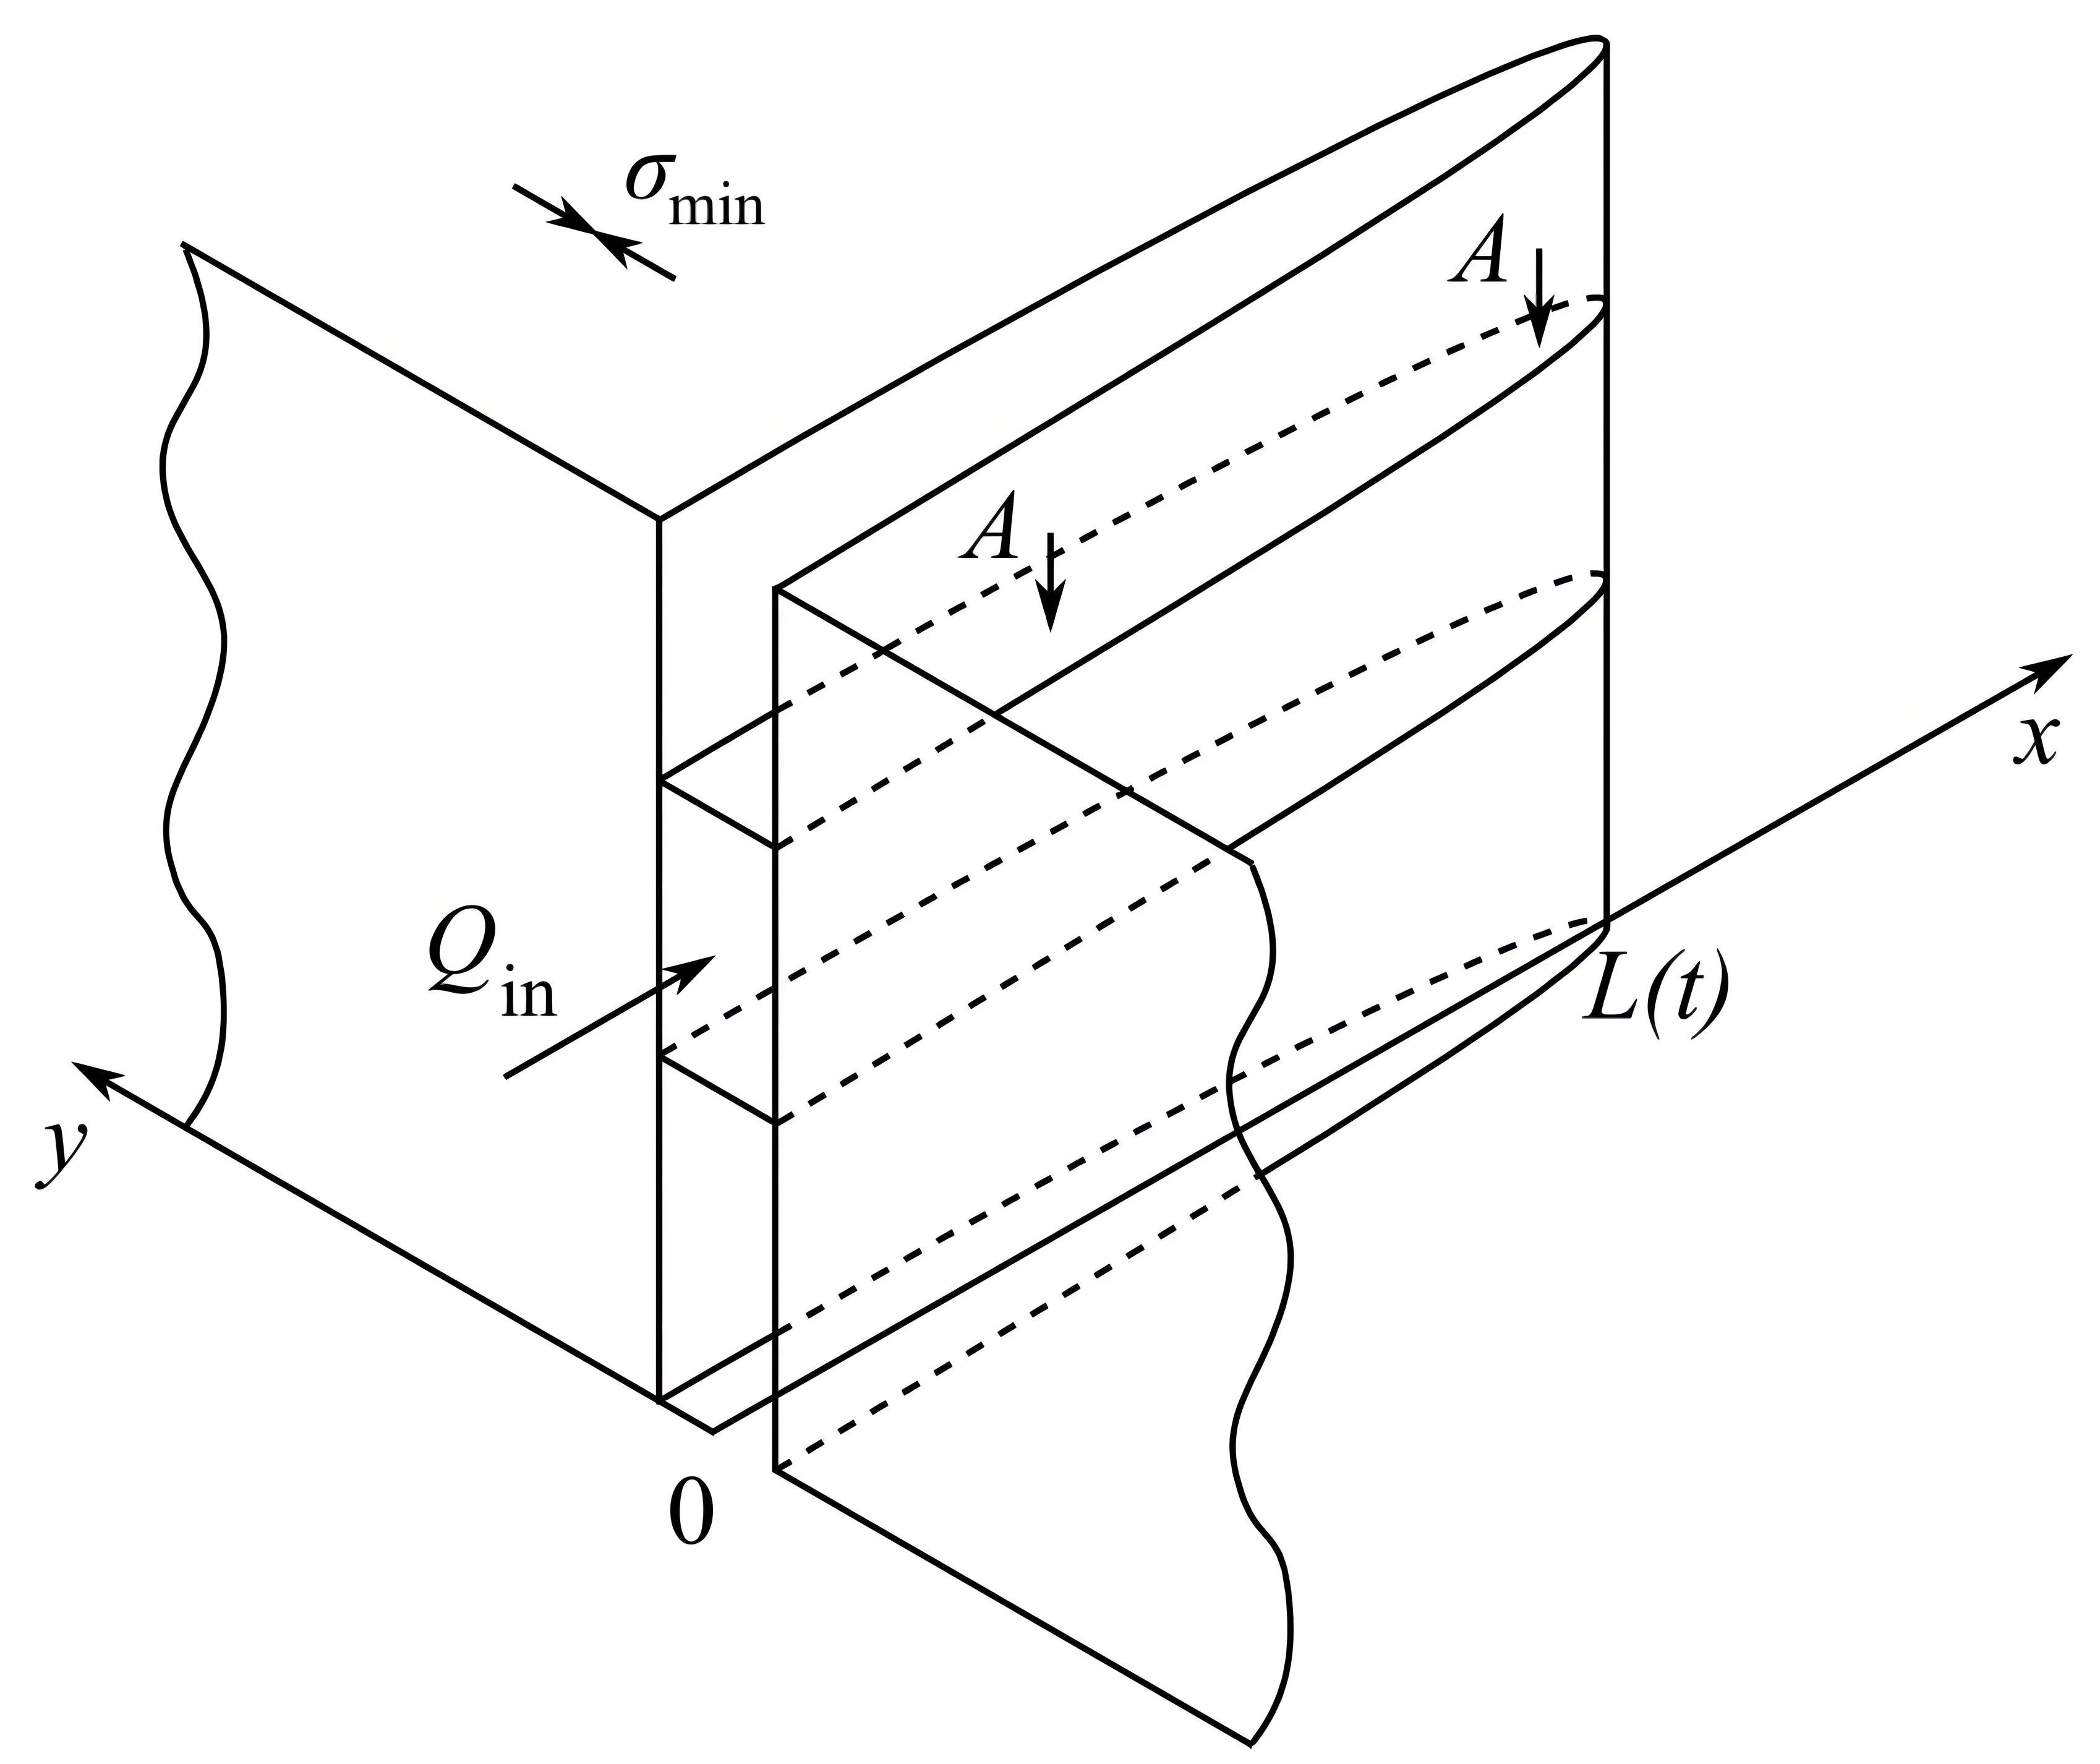
\includegraphics[width=6cm]{kgd_model_3D.jpg}
\end{textblock*}

\begin{textblock*}{8cm}(6.5cm,6.1cm)
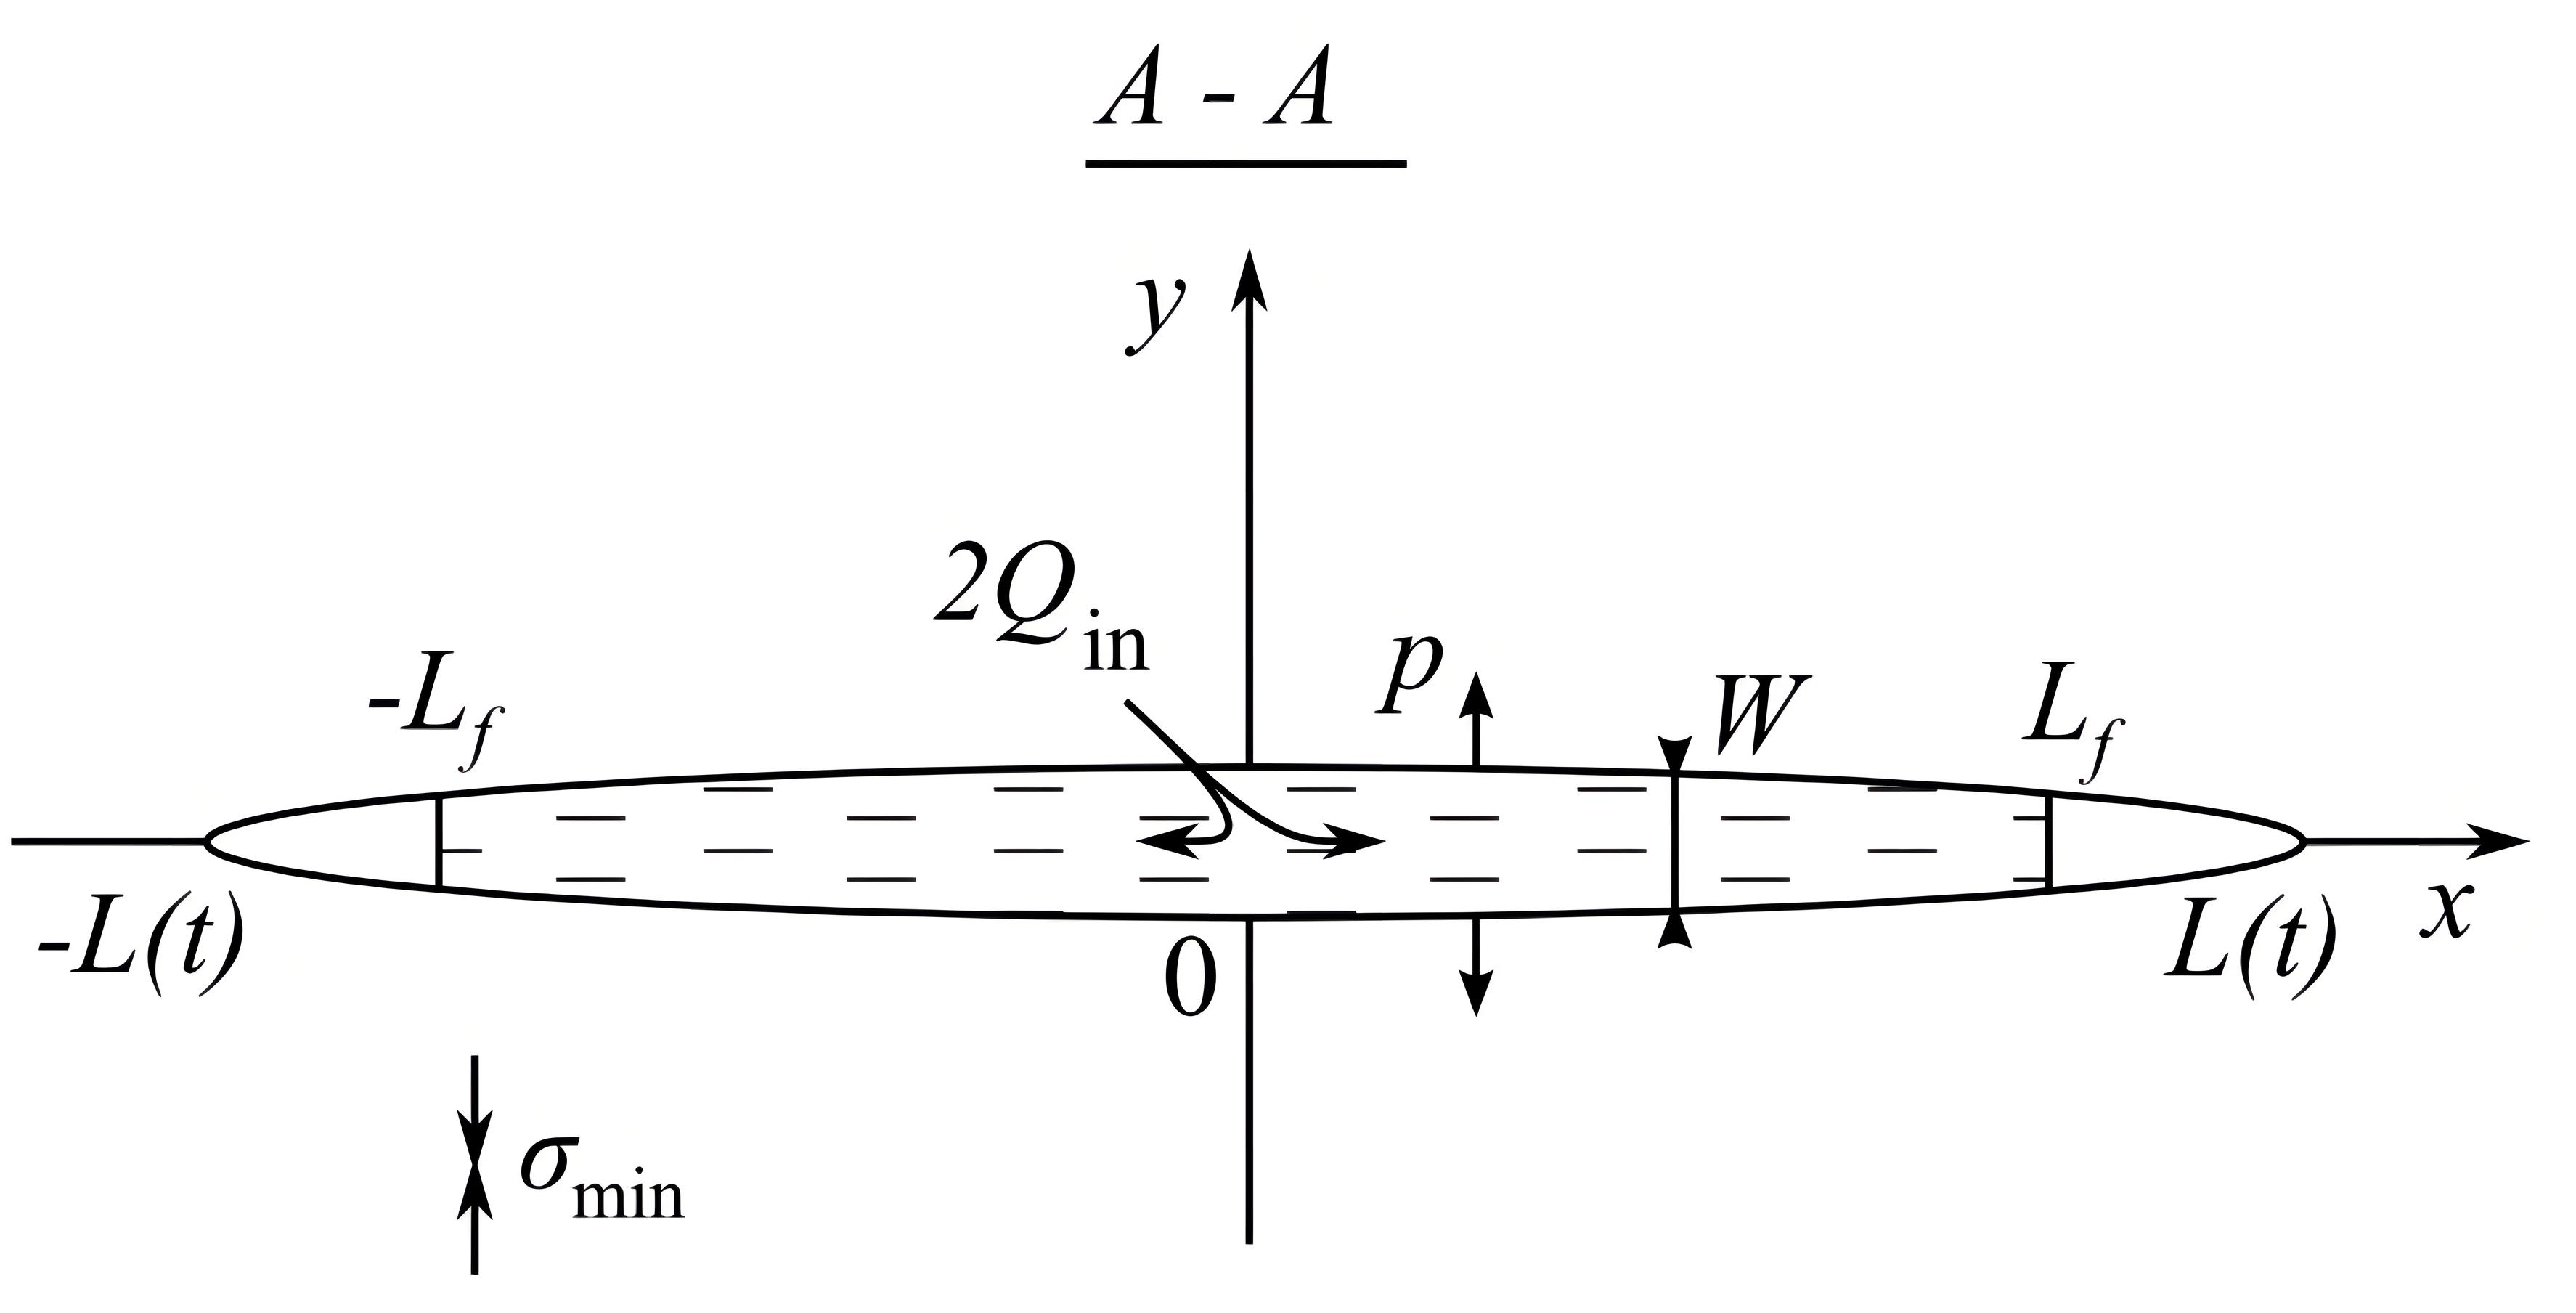
\includegraphics[width=6cm]{kgd_model_A-A_plane.jpg}
\end{textblock*}

\begin{textblock*}{6cm}(0.5cm,8.7cm)
\tiny
\textcolor{lit_gray}{E.V. Dontsov. An approximate solution for a plane strain hydraulic fracture that accounts for fracture toughness, fluid viscosity, and leak-off. \emph{Int. J. Fract.}, 205:221-237, 2017}
\end{textblock*}

\normalsize

\end{frame}

\begin{frame}
\frametitle{Модель радиальной трещины}

\scriptsize

\begin{textblock*}{7cm}(0.5cm,0.8cm)
$$
\begin{cases}
\dfrac{\partial w}{\partial t}+\dfrac{1}{r}\dfrac{\partial}{\partial r}\!\left(rq\right)+\dfrac{C'}{\sqrt{t-t_0(r)}}=Q_0\delta(r),\\[15pt]
q=-\dfrac{w^3}{\mu'}\dfrac{\partial p_n}{\partial r},\\[5pt]
p_n(r,t)=-\dfrac{E'}{2\pi R}\displaystyle\int\limits_{0}^{R(t)}M\!\left(\dfrac{r}{R},\dfrac{r'}{R}\right)\dfrac{\partial w(r',t)}{\partial r'}dr',\\[20pt]
\displaystyle\lim_{r\to R}\dfrac{w}{(R-r)^{1/2}}=\dfrac{K'}{E'},
\end{cases}
$$
где $C'=2C_l$; $\,\,\,\mu'=12\mu$; $\,\,\,E'=\dfrac{E}{1-\nu^2}$; $\,\,\,K'=\dfrac{8K_{Ic}}{\sqrt{2\pi}}$;
$$
M(\rho,s)=
\begin{cases}
\dfrac{1}{\rho}\,K\!\left(\dfrac{s^2}{\rho^2}\right)+\dfrac{\rho}{s^2-\rho^2}\,E\!\left(\dfrac{s^2}{\rho^2}\right)\\\ \\
\dfrac{s}{s^2-\rho^2}\,E\!\left(\dfrac{\rho^2}{s^2}\right)
\end{cases}
$$
\end{textblock*}

\begin{textblock*}{7cm}(7cm,1cm)
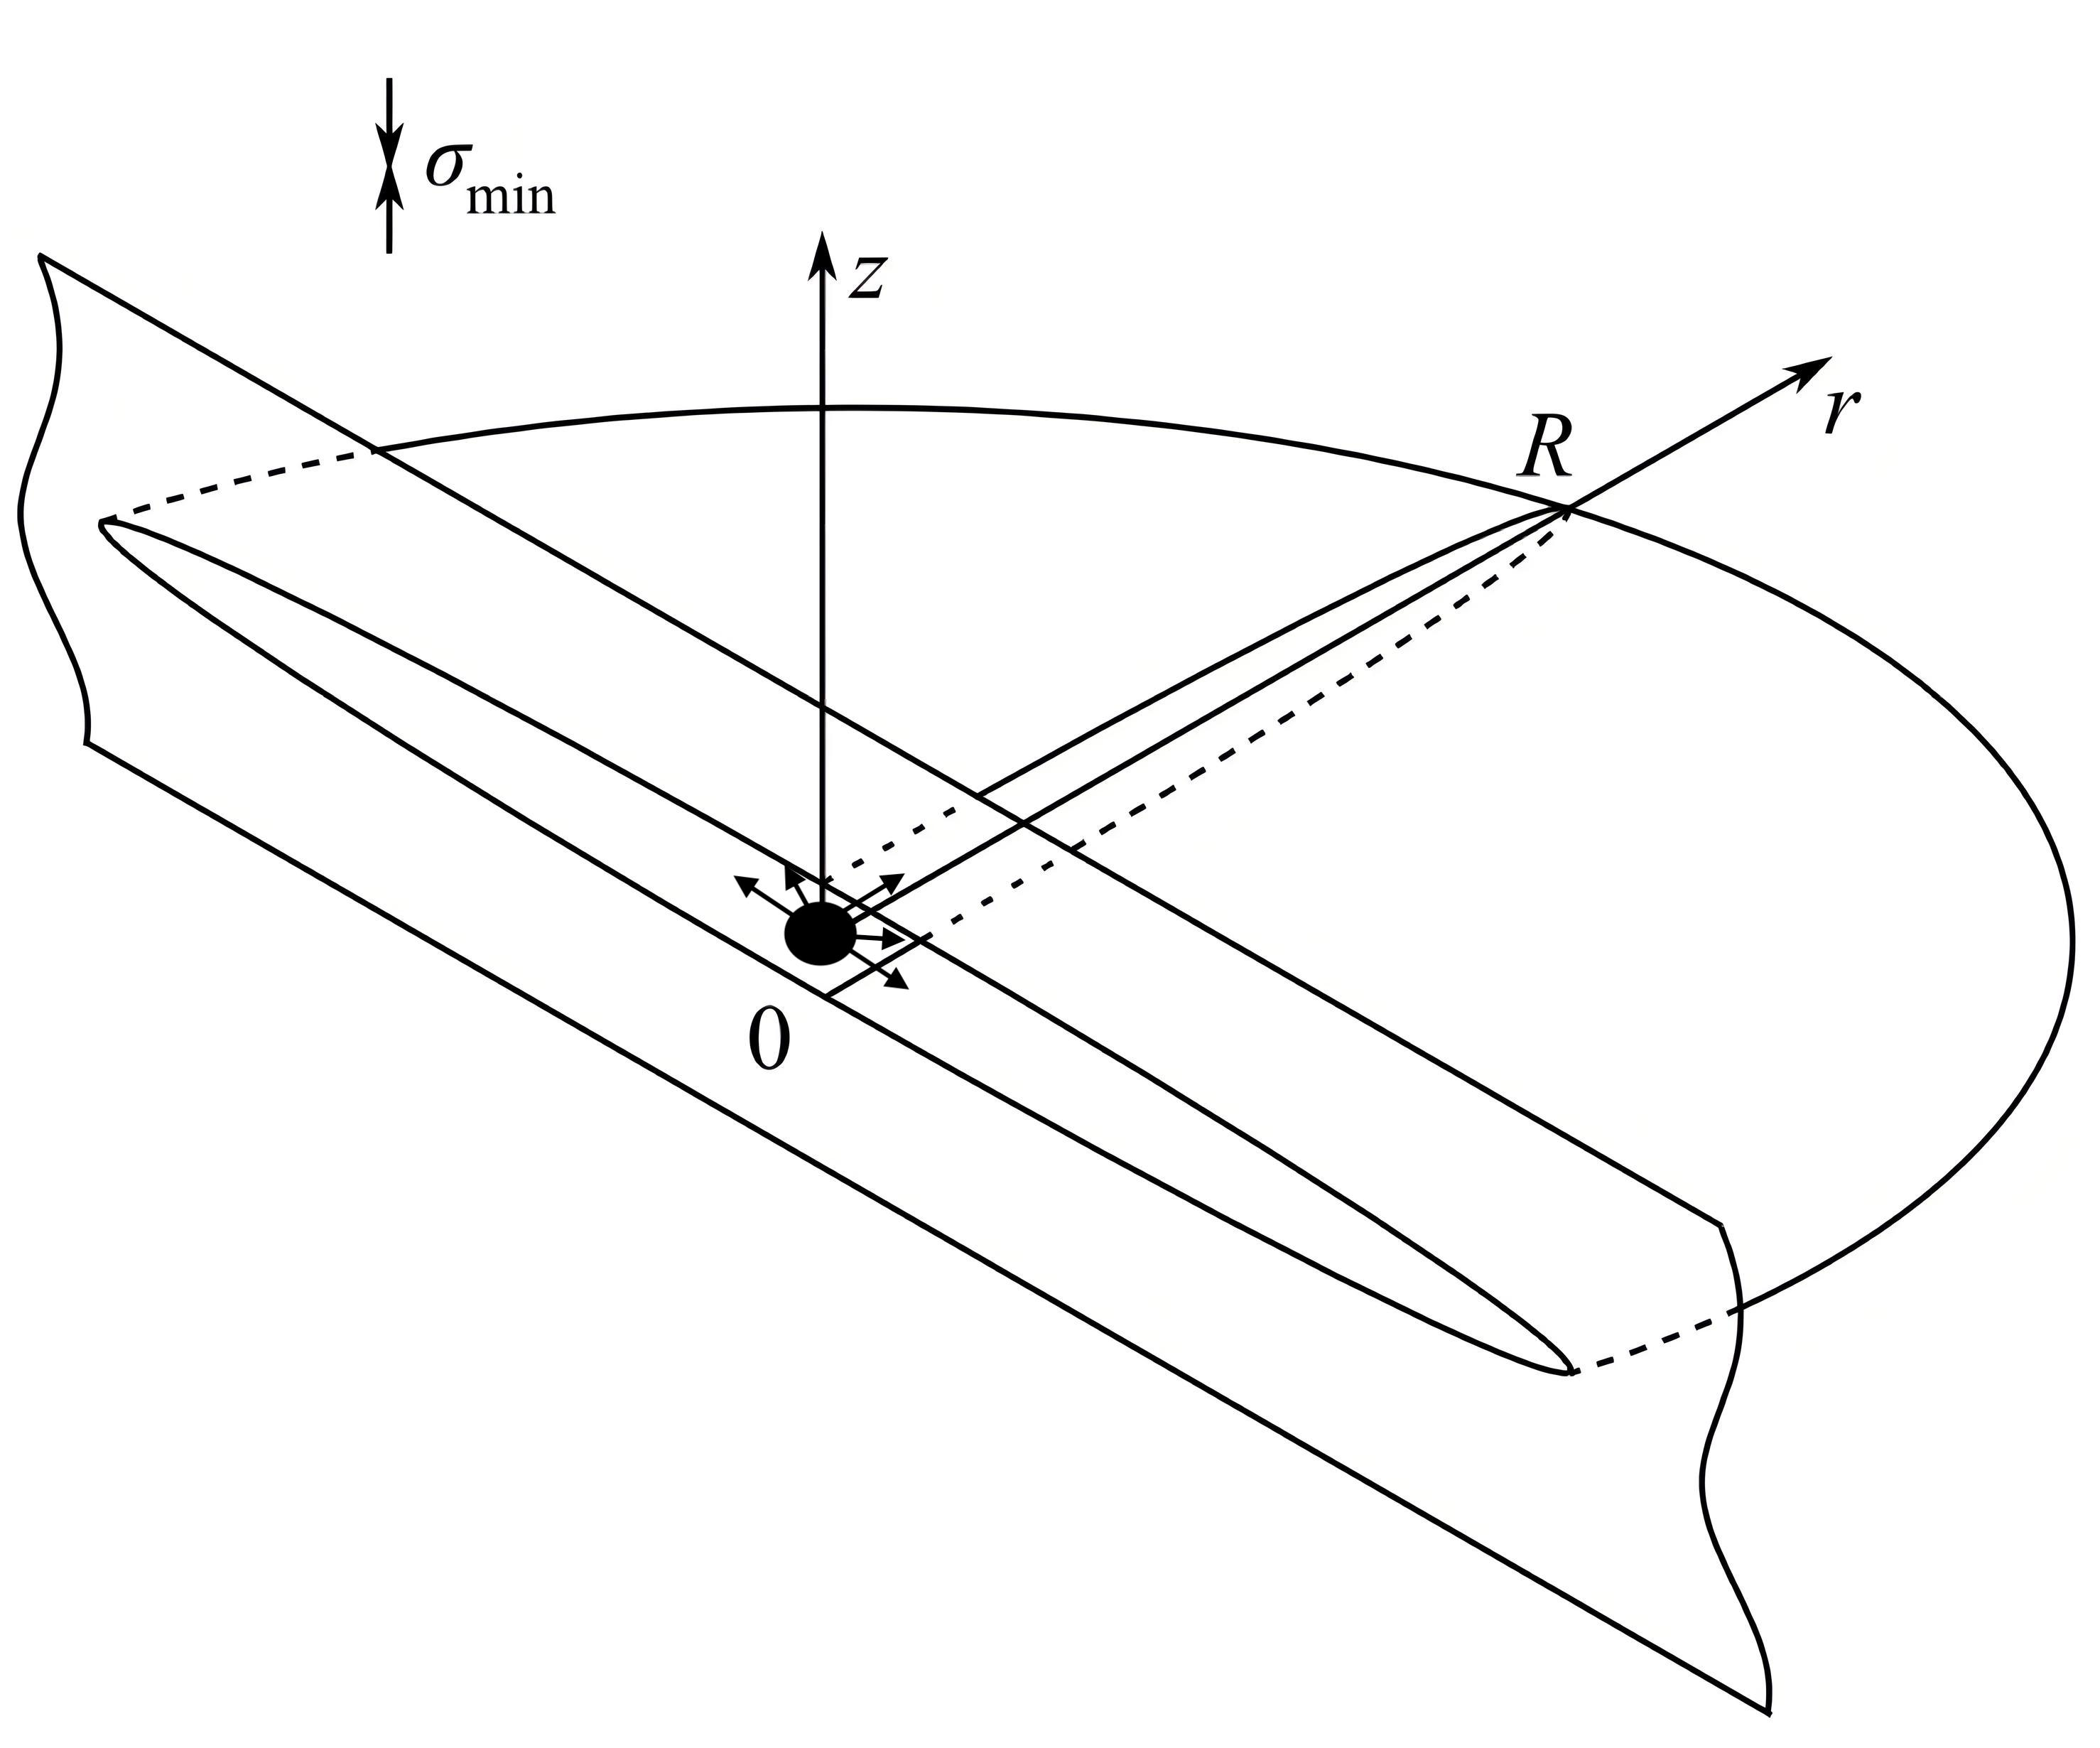
\includegraphics[width=5.5cm]{radial_model_3D.jpg}
\end{textblock*}

\begin{textblock*}{7cm}(7.4cm,5.7cm)
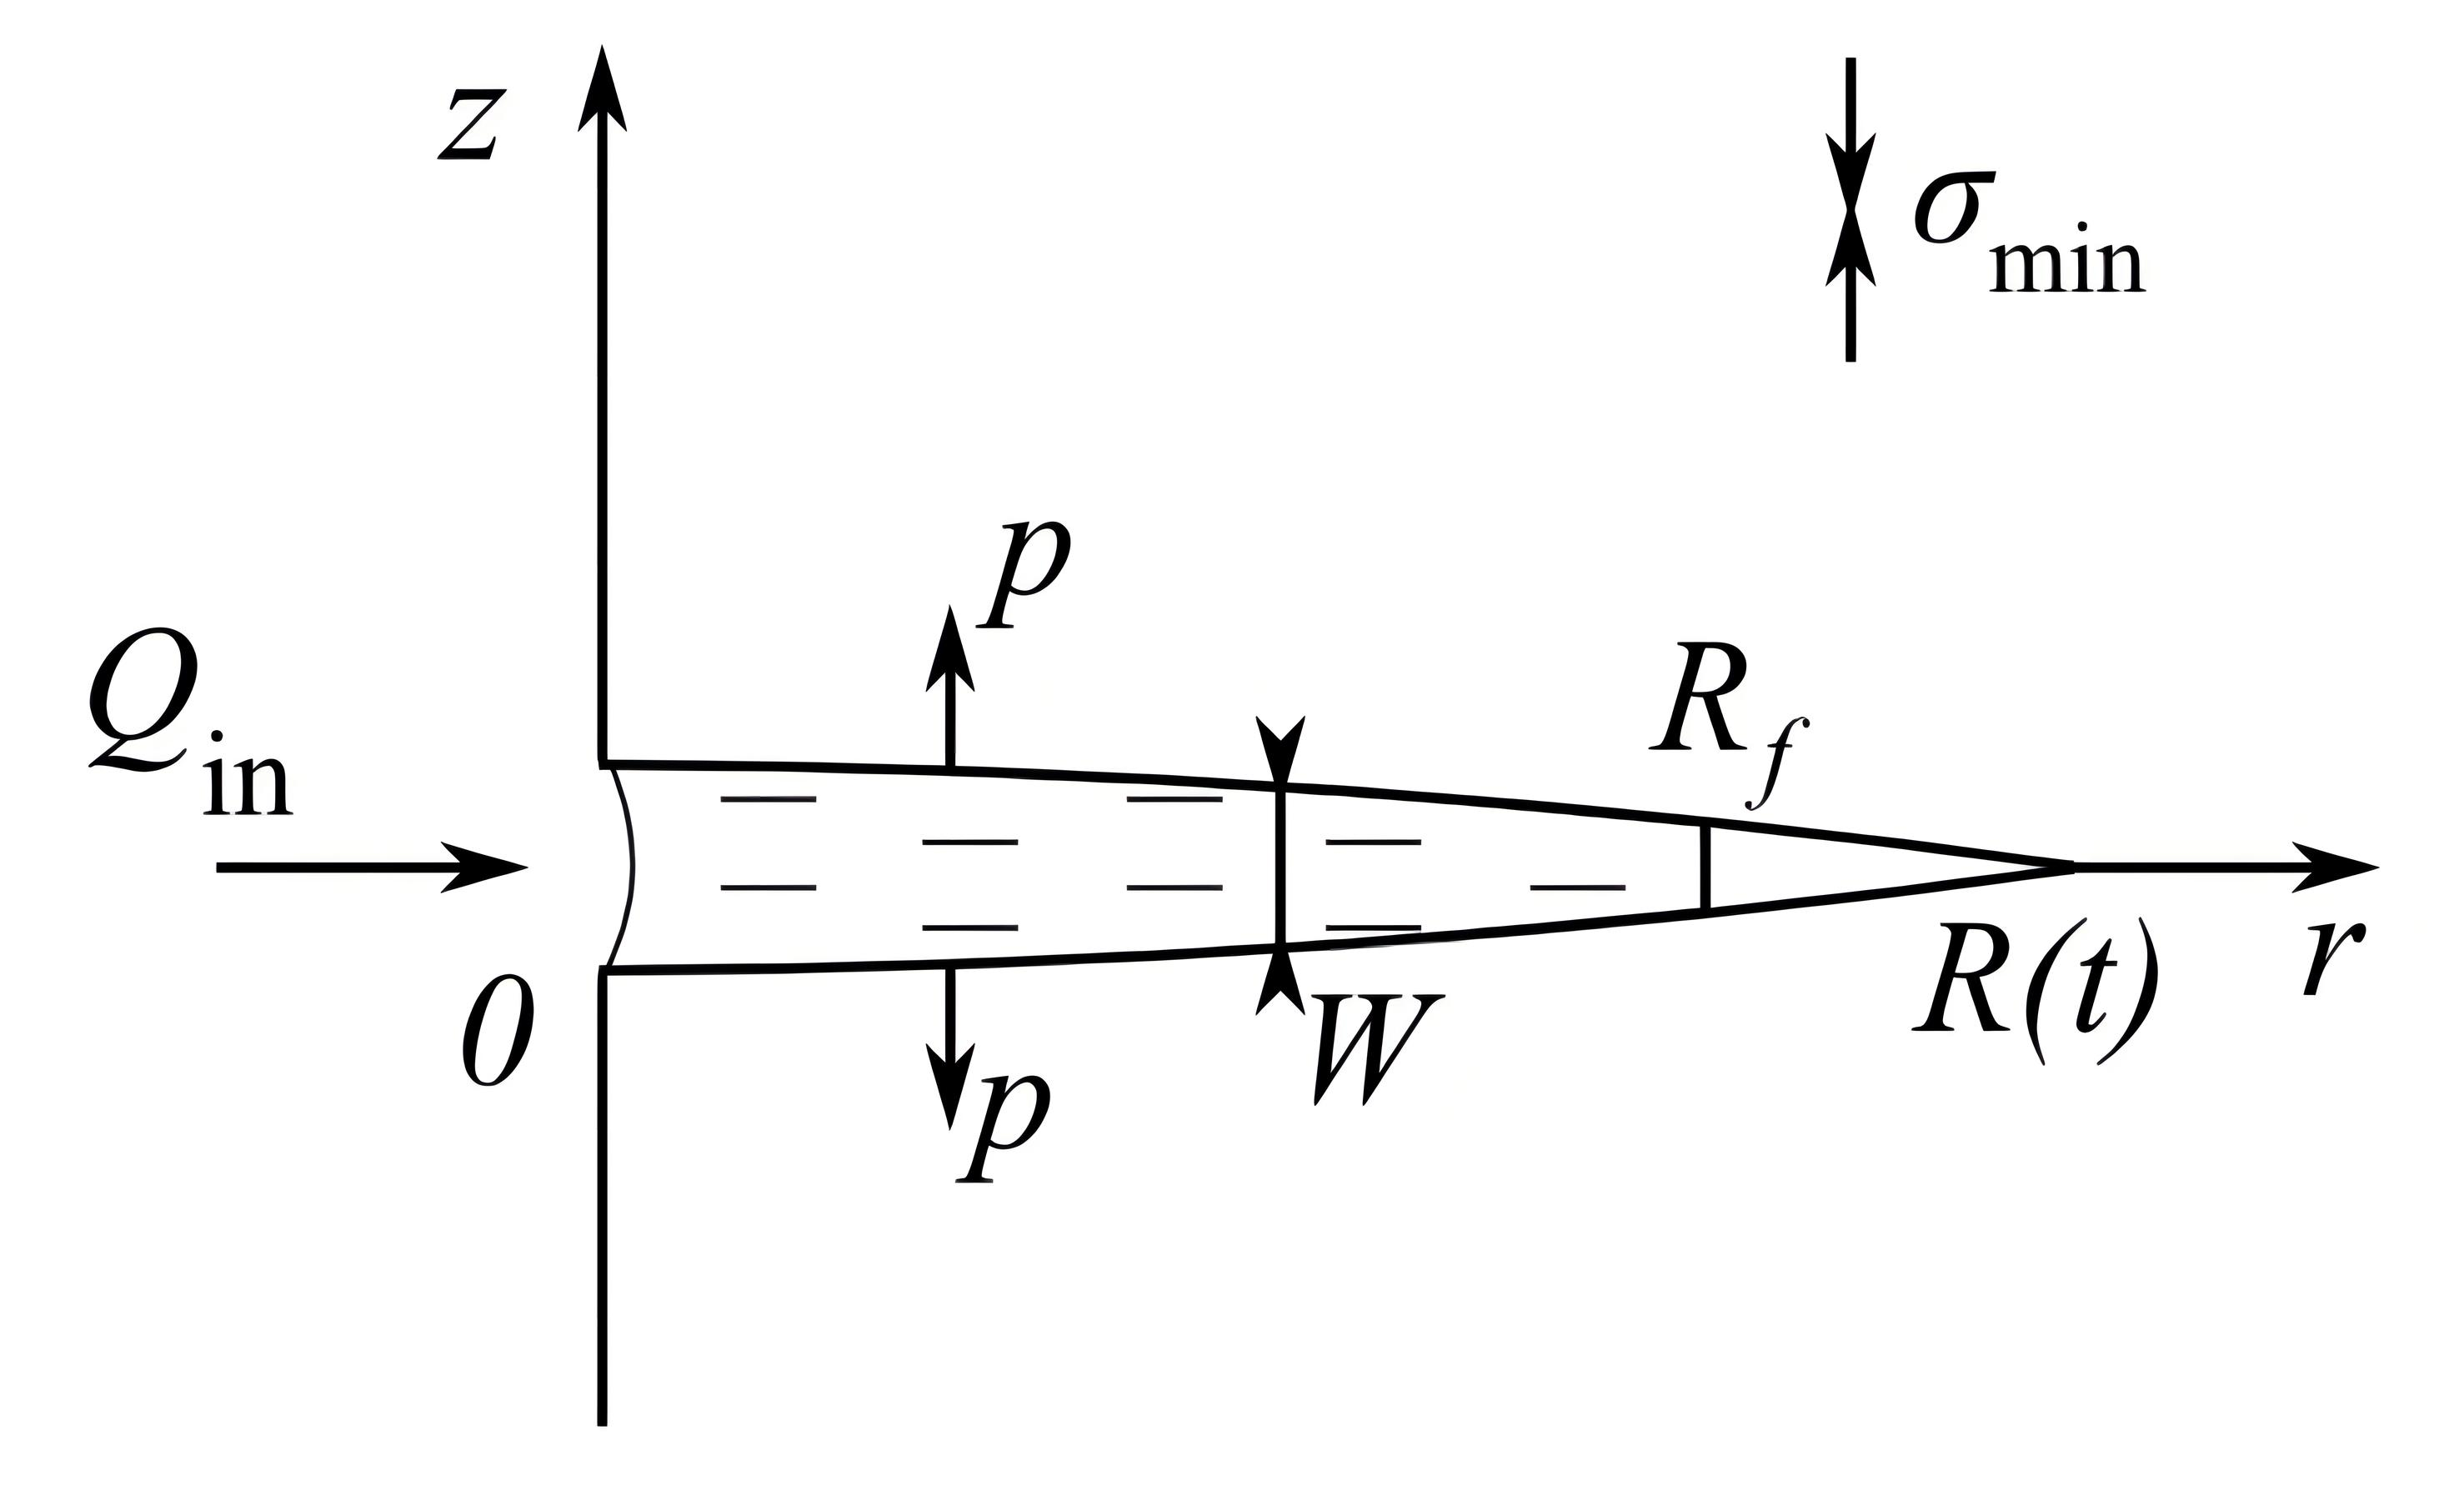
\includegraphics[width=5.2cm]{radial_model_A-A_plane.jpg}
\end{textblock*}

\begin{textblock*}{6cm}(0.5cm,8.7cm)
\tiny
\textcolor{lit_gray}{E.V. Dontsov. An approximate solution for a penny-shaped hydraulic fracture that accounts for fracture toughness, fluid viscosity, and leak-off. \emph{R. Soc. Open Sci.}, 3:160737, 2016}
\end{textblock*}

\normalsize

\end{frame}


\begin{frame}
\frametitle{Модель Перкинса-Керна-Нордгрена (модель PKN)}

\scriptsize

\begin{textblock*}{7cm}(0.5cm,1.2cm)
$$
\begin{cases}
\dfrac{\partial\bar{w}}{\partial t}+\dfrac{\partial\bar{q}_x}{\partial x}+\dfrac{C'}{\sqrt{t-t_0(x)}}=\dfrac{Q_0}{H}\delta(x),\\[15pt]
\bar{q}_x=-\dfrac{\bar{w}^3}{\pi^2\mu}\dfrac{\partial p_n}{\partial x},\\[15pt]
p_n(x,t)=\dfrac{2E'}{\pi^2H}\displaystyle\int\limits_{-L(t)}^{L(t)}\bar{w}(x',t)\dfrac{dG(2(x'-x)/H)}{dx'}dx',\\[22pt]
\displaystyle\lim_{x\to L}\dfrac{w}{(L-x)^{1/2}}=\dfrac{K'}{E'},
\end{cases}
$$
где $C'=2C_l$; $\,\,\,\mu'=12\mu$; $\,\,\,E'=\dfrac{E}{1-\nu^2}$; $\,\,\,K'=\dfrac{8K_{Ic}}{\sqrt{2\pi}}$;
$$
G(s)=\frac{\sqrt{1+s^2}}{s}\,E\!\left(\frac{1}{1+s^2}\right)
$$
\end{textblock*}

\begin{textblock*}{7cm}(7.4cm,1cm)
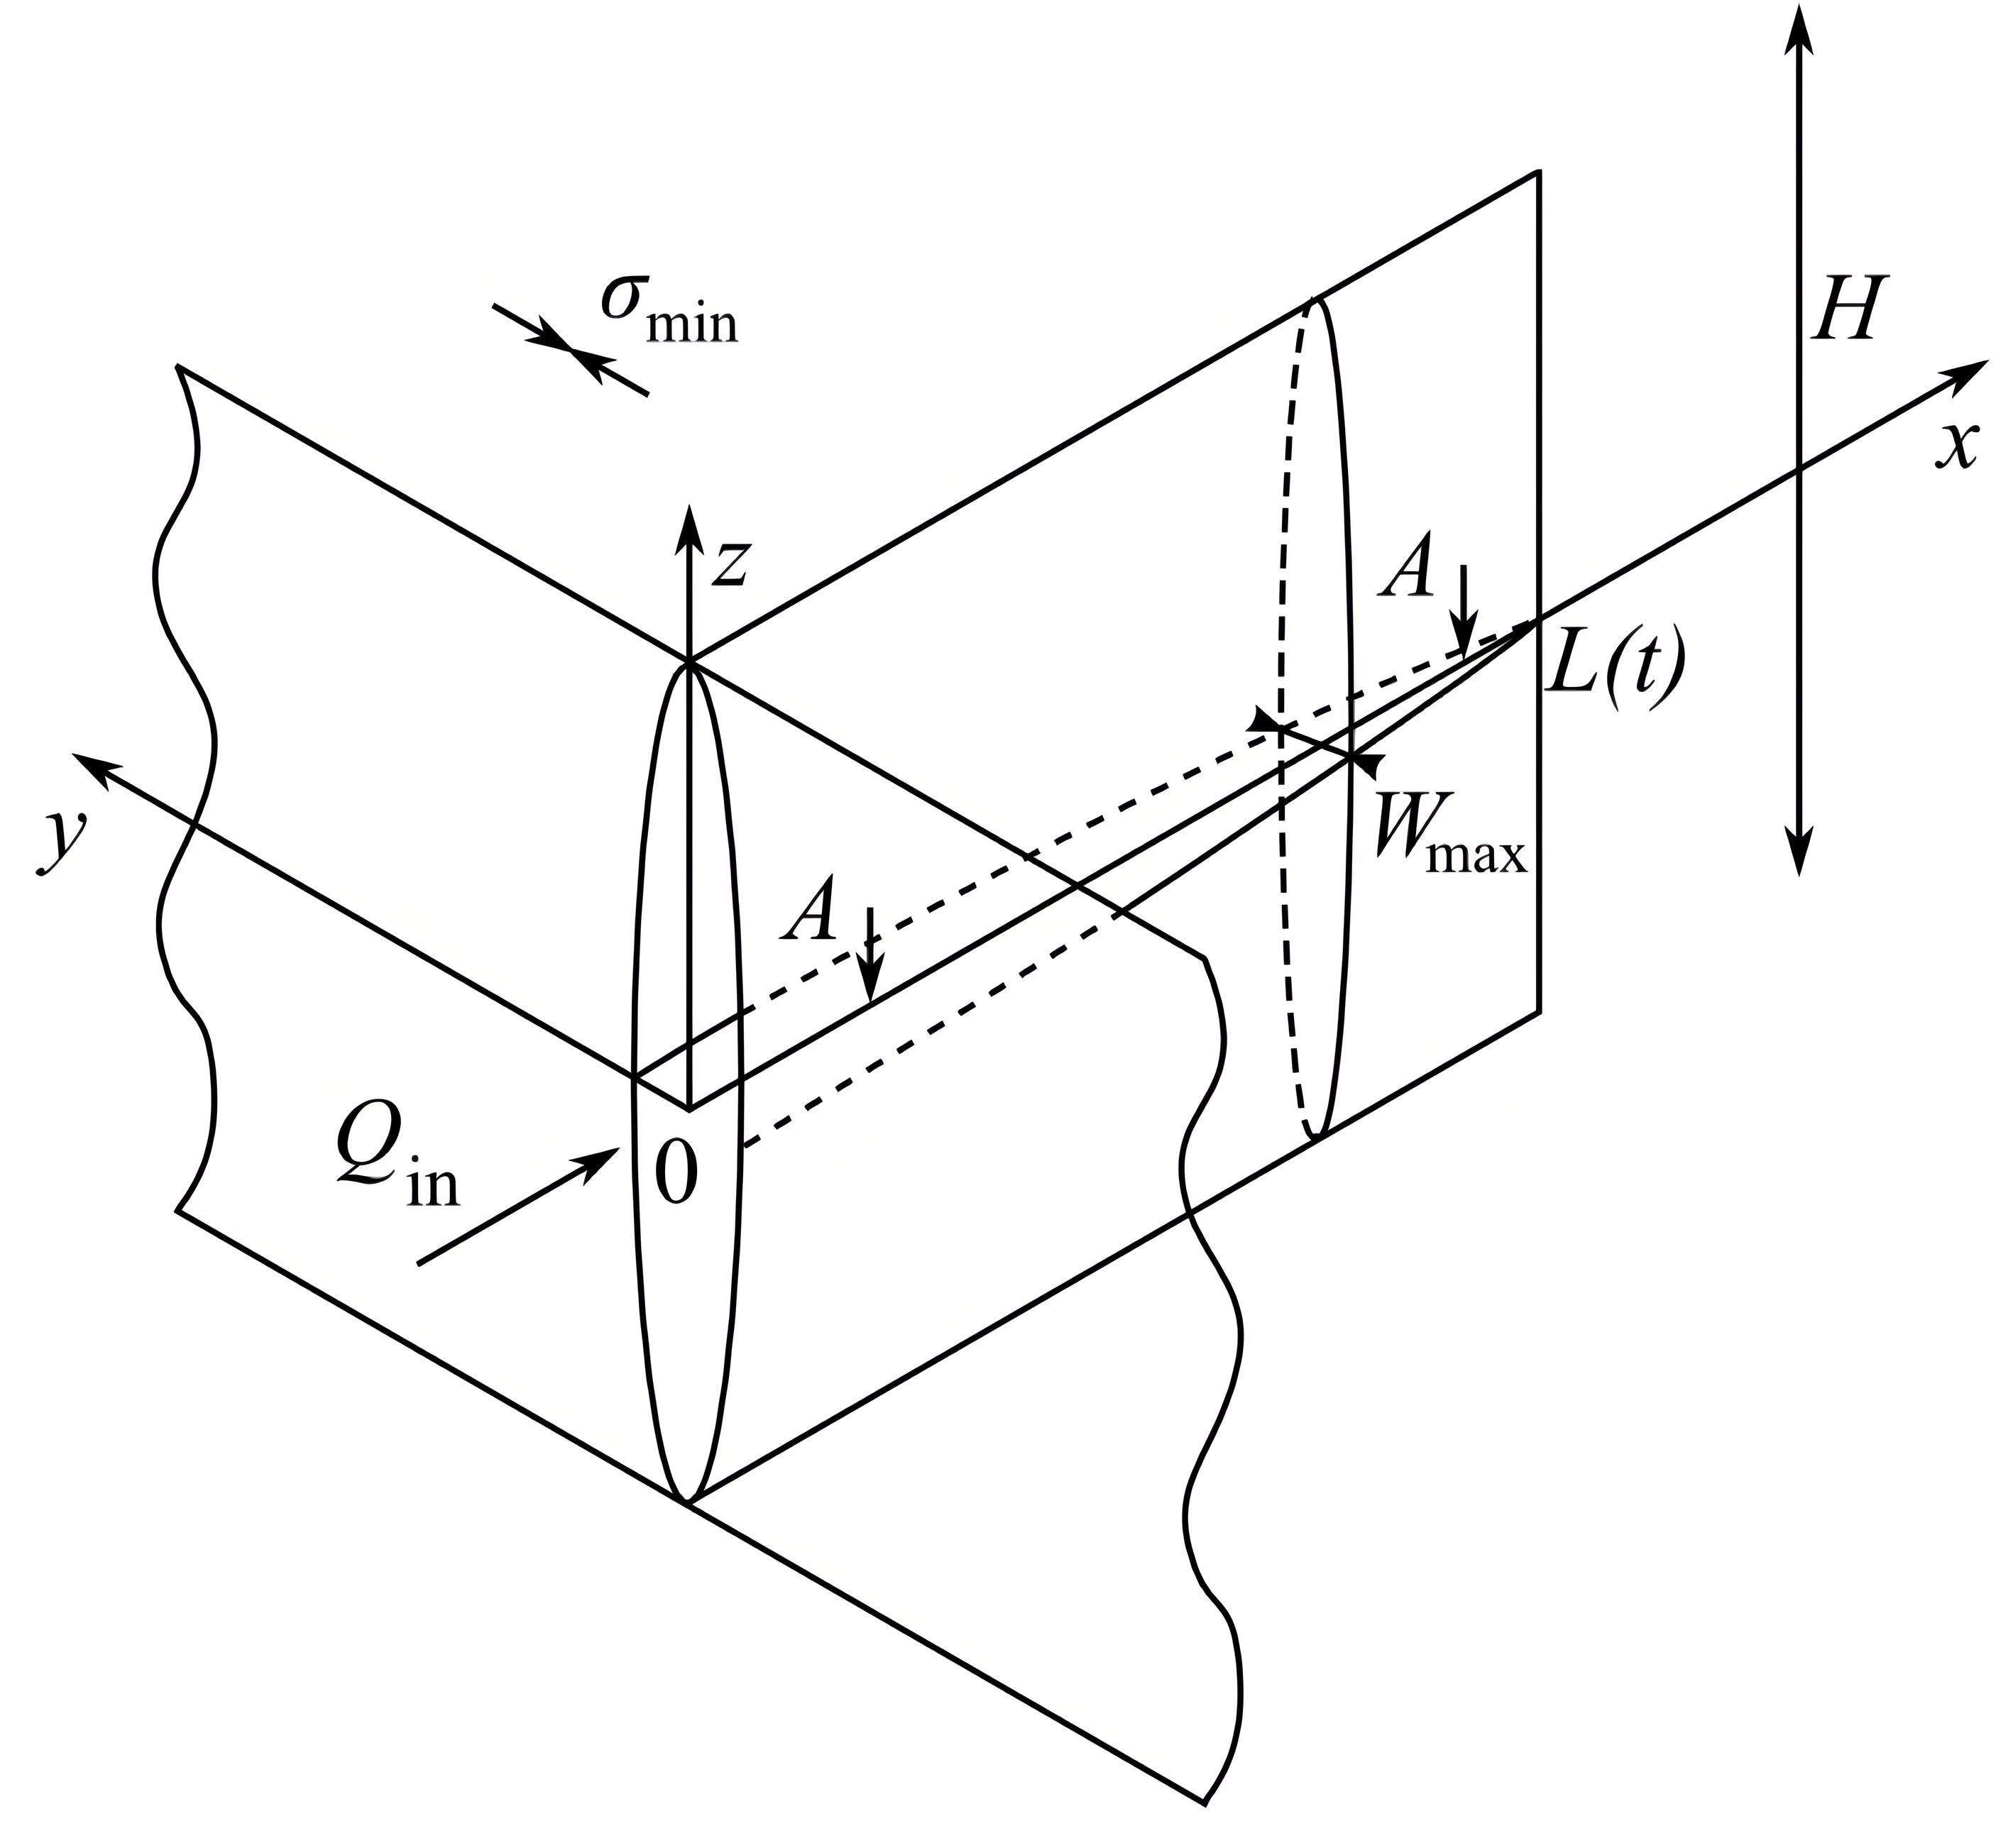
\includegraphics[width=5.2cm]{pkn_model_3D.jpg}
\end{textblock*}

\begin{textblock*}{7cm}(7.5cm,6.3cm)
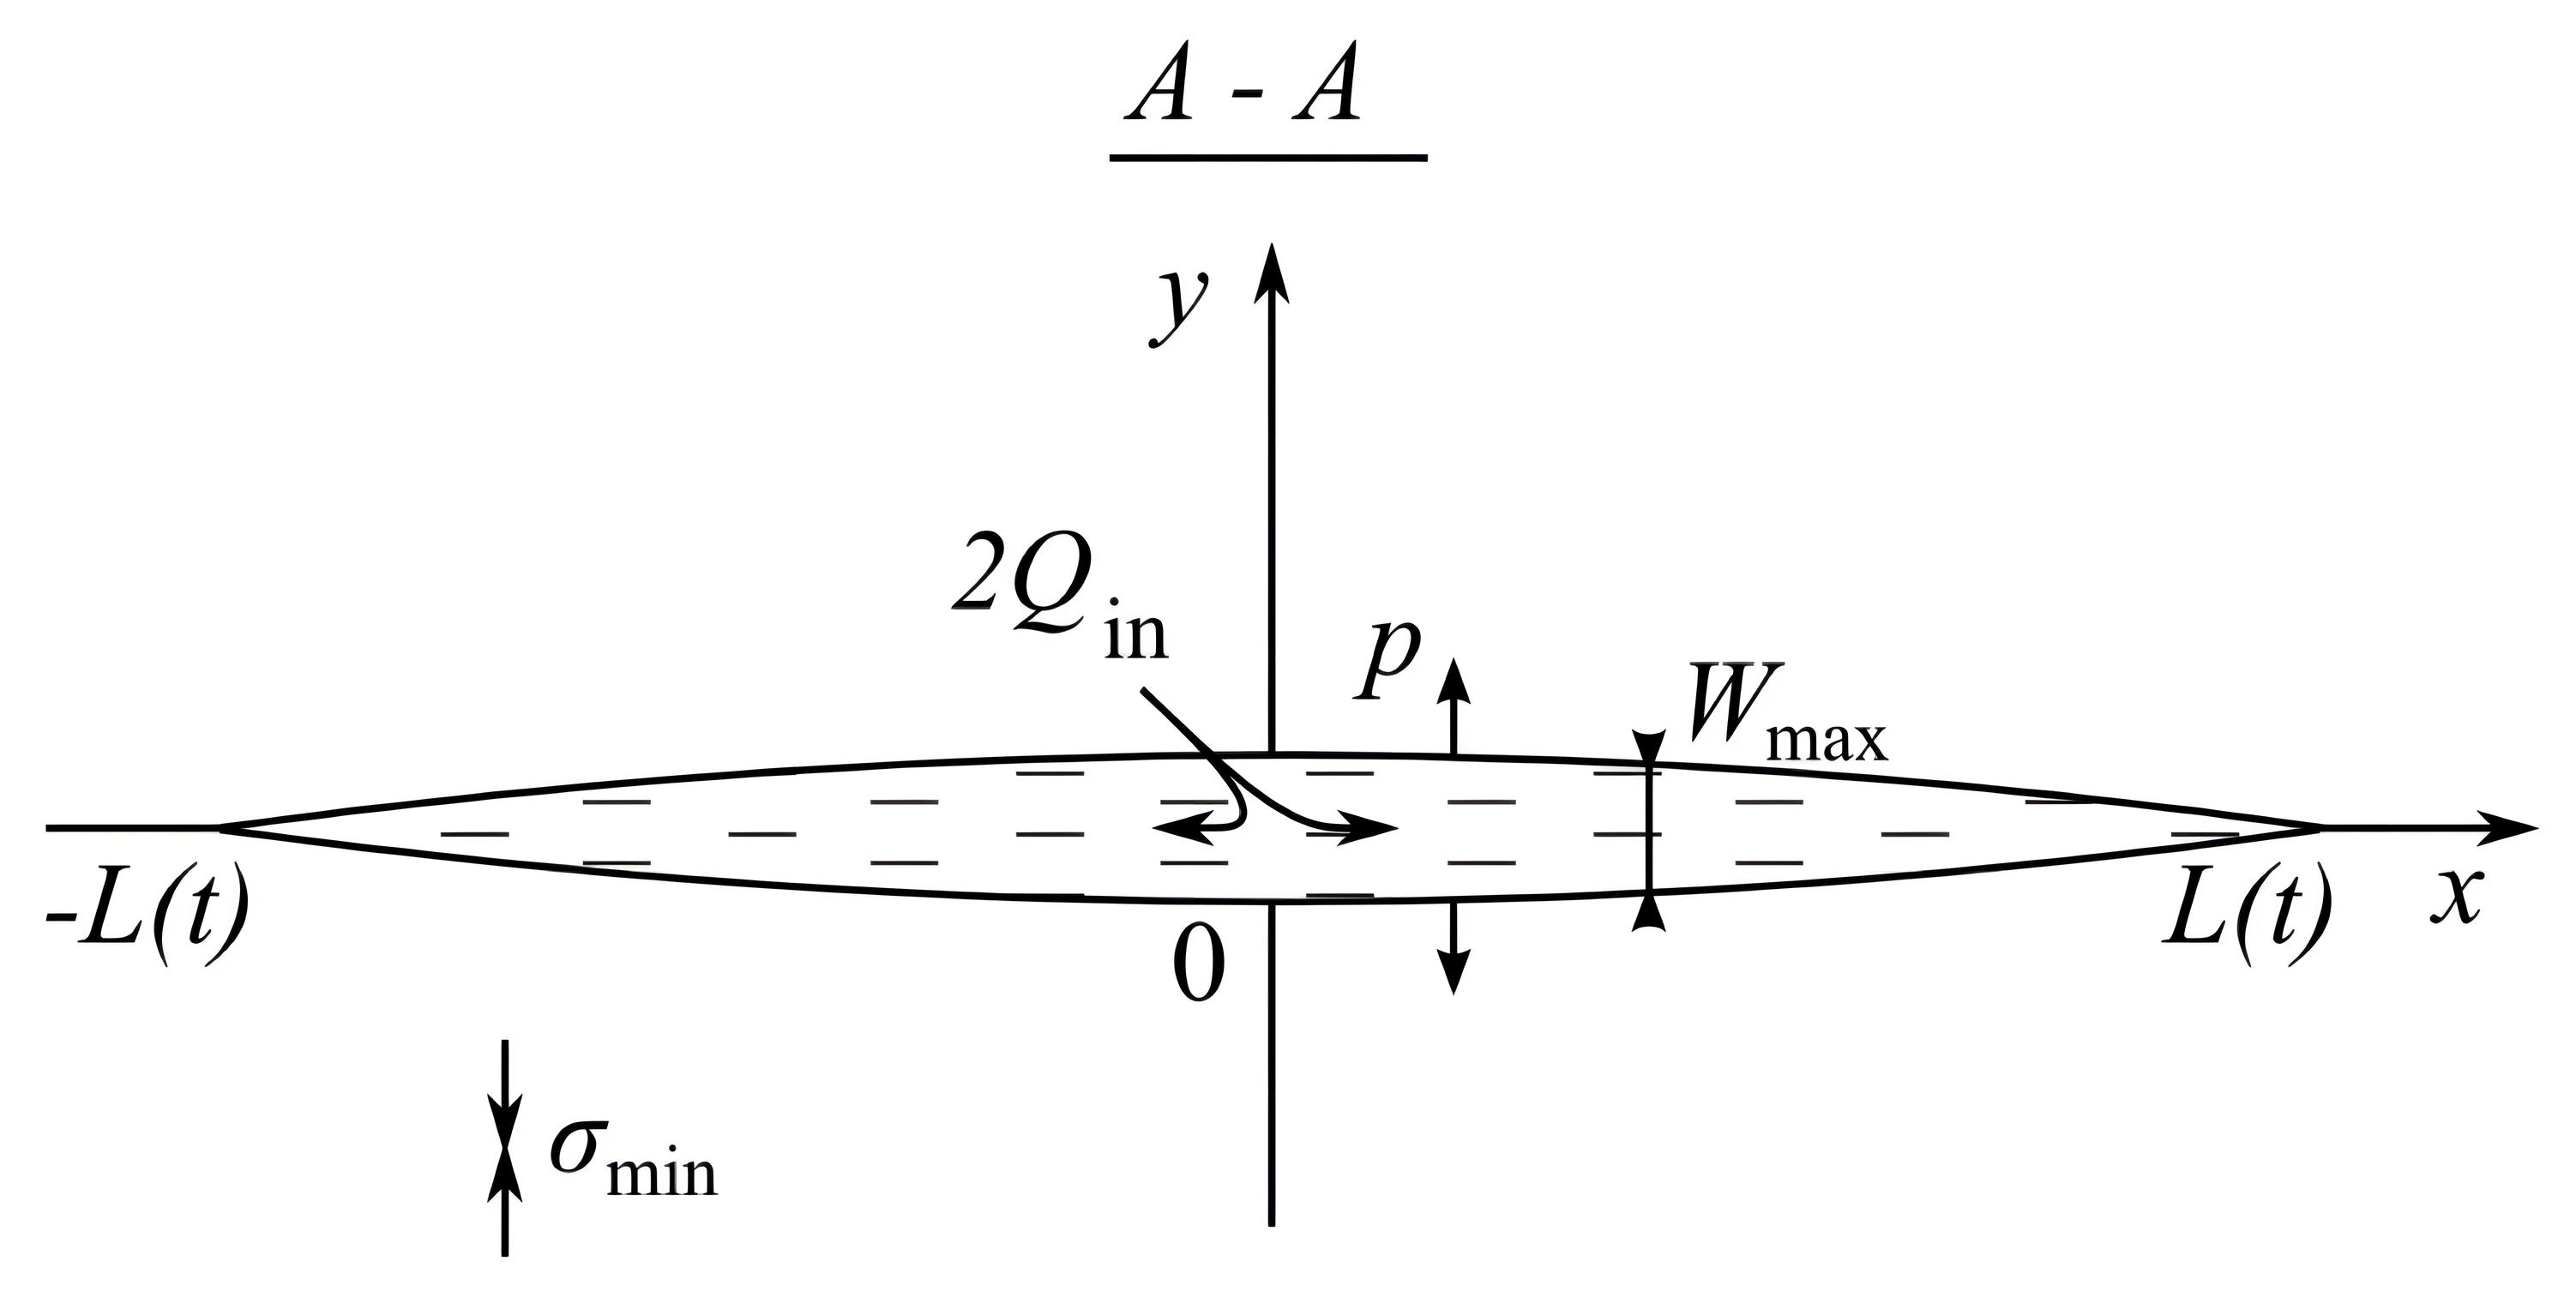
\includegraphics[width=5cm]{pkn_model_A-A_plane.jpg}
\end{textblock*}

\begin{textblock*}{6cm}(0.5cm,8.9cm)
\tiny
\textcolor{lit_gray}{E.V. Dontsov. Analysis of a constant height hydraulic fracture, arXiv:2110.13088v1 [physics.geo-ph], 25 Oct 2021}
\end{textblock*}

\normalsize

\end{frame}


\begin{frame}
\frametitle{Асимптотические решения модели PKN}

\end{frame}


\begin{frame}
\frametitle{Модель трещины автоГРП = модель PKN в случае доминирования утечек}

\end{frame}


\begin{frame}
\frametitle{Схема перераспределения потоков между трещинами гидроразрыва и законы Кирхгофа}

\begin{textblock*}{11cm}(1cm,1.5cm)
%\tiny Подпись к рисунку
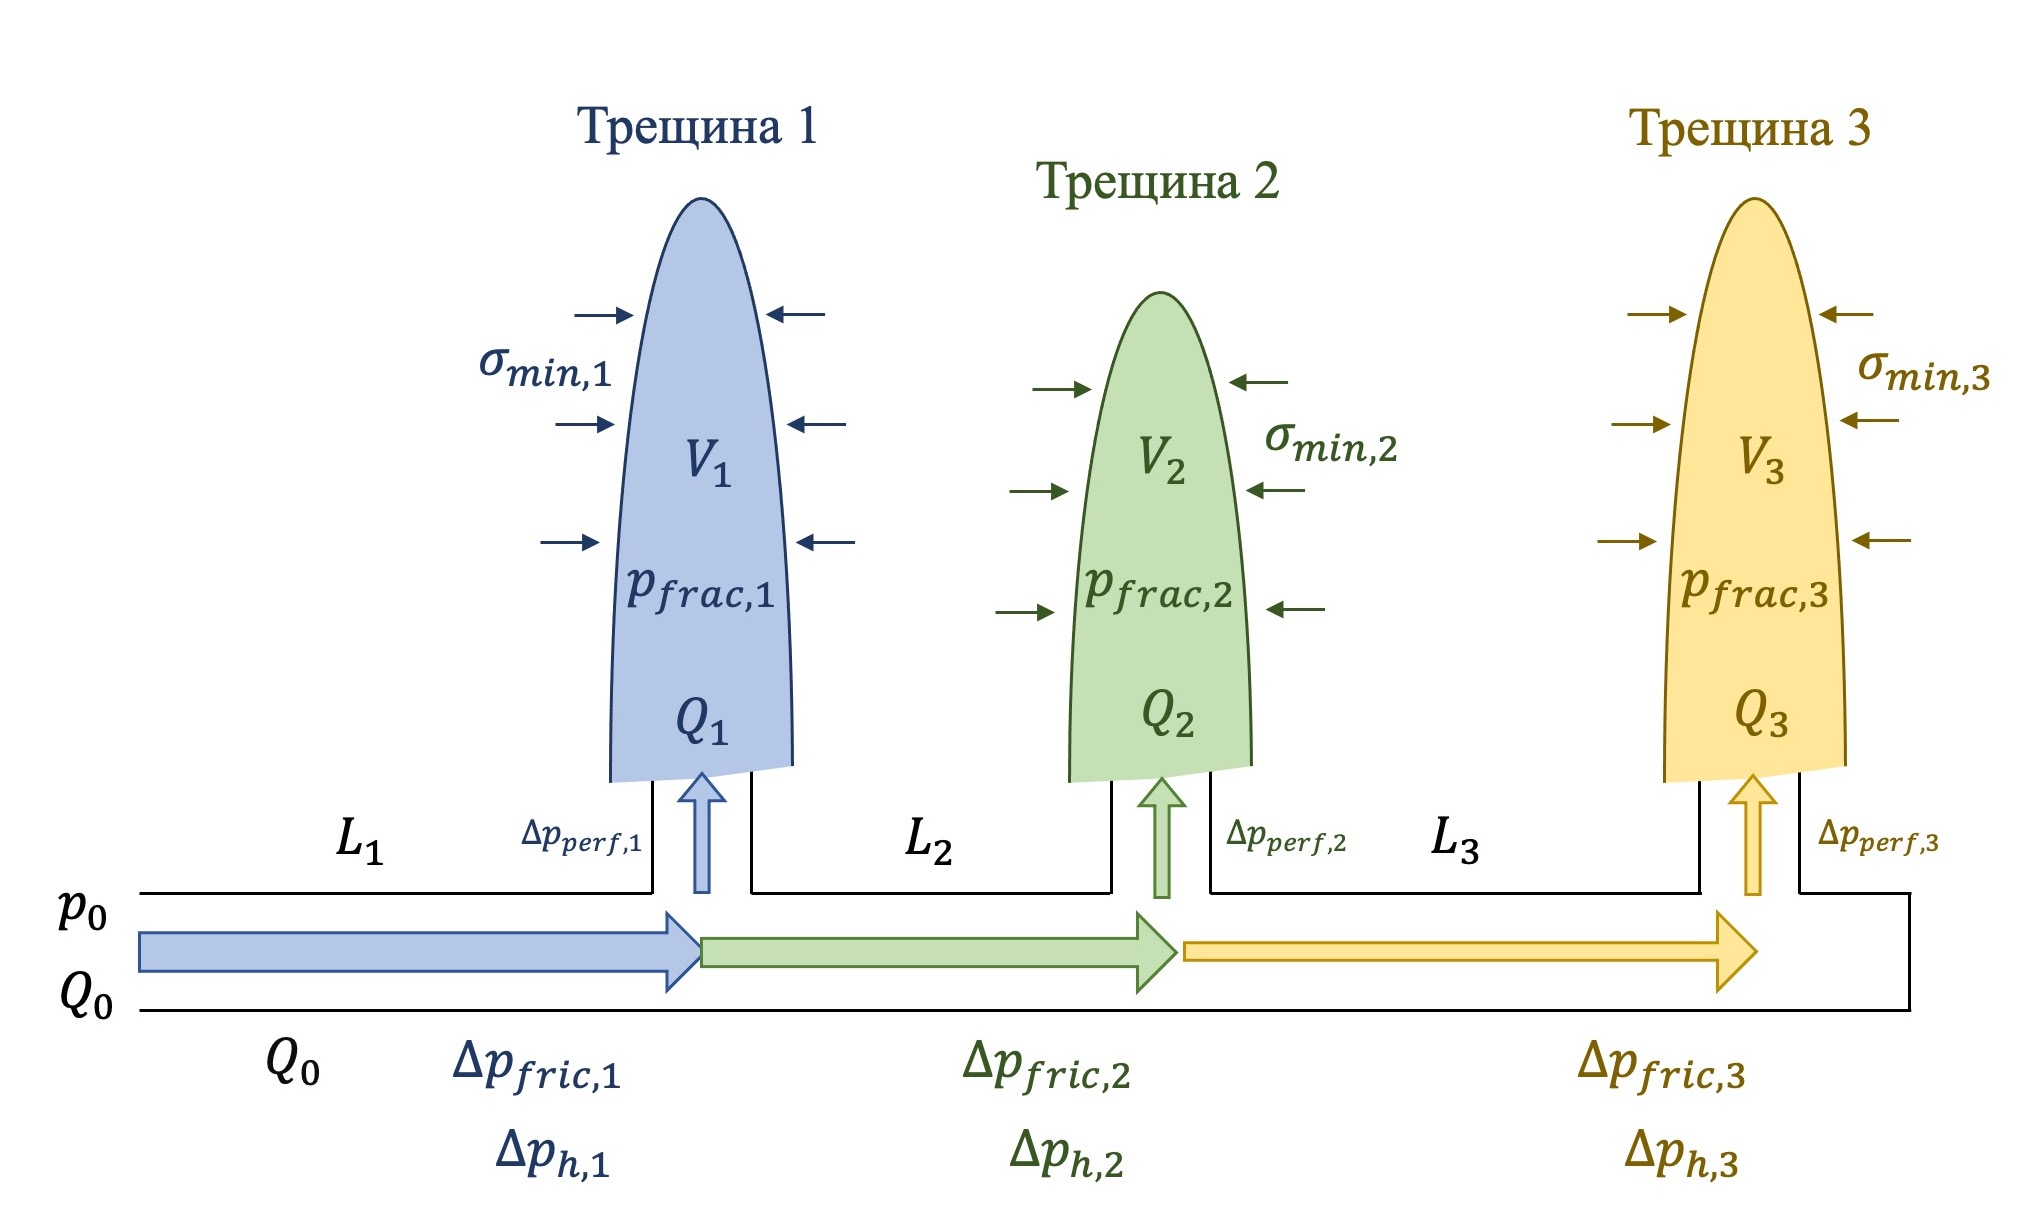
\includegraphics[width=10cm]{flow_distribution_scheme.jpg}
\end{textblock*}

\begin{textblock*}{4cm}(-0.5cm,7.5cm)
$$\boxed{Q_0=\sum\limits_{i=1}^{N}Q_i}$$
\end{textblock*}

\begin{textblock*}{11cm}(2.2cm,7.5cm)
$$\boxed{p_0=\sigma_{\text{min},i}+p_{\text{net},i}+\Delta p_{\text{perf},i}-\sum_{j=1}^{i}{\Delta p_{h,\,j}}+\sum_{j=1}^{i}\Delta p_{\text{fric},\,j}}$$
\end{textblock*}

\end{frame}


\begin{frame}
\frametitle{Чистое давление в трещинах PKN}

\end{frame}


\begin{frame}
\frametitle{Падение давления на перфорациях}

\end{frame}


\begin{frame}
\frametitle{Падение давления на трение}

\end{frame}


\begin{frame}
\frametitle{Запись законов Кирхгофа в векторной форме}

Вектор неизвестных:
$$Q^T=\left[Q_1,Q_2,...,Q_N,p_0\right]$$

Вектор невязок:
$$\left[F_1,F_2,...,F_N,F_{N+1}\right],$$
где
$$
F_i=
\begin{cases}
\sigma_{\text{min},i}+p_{\text{net},i}+\Delta p_{\text{perf},i}-\sum\limits_{j=1}^{i}{\Delta p_{h,j}}+\sum\limits_{j=1}^{i}{\Delta p_{\text{fric},j}}-p_0\\\,\,\,\,\,\,\,\,\,\,\,\,\,\,\,\,\,\,\,\,\,\,\,\,\,\,\,\,\,\,\,\,\left(\text{при }i\leqslant N\right)\\\ \\
Q_0-\sum\limits_{j=1}^{N}{Q_j}\left(\text{при }i=N+1\right)
\end{cases}
$$

\end{frame}


\begin{frame}
\frametitle{Итеративная процедура решения}
Матрица Якоби:
$$J = \begin{bmatrix}
	\dfrac{\partial F_1}{\partial Q_1} & \dots & \dfrac{\partial F_1}{\partial Q_N} & \dfrac{\partial F_1}{\partial p_0} \\
	\vdots & \ddots & \vdots & \vdots \\
	\dfrac{\partial F_{N+1}}{\partial Q_1} & \dots & \dfrac{\partial F_{N+1}}{\partial Q_N} & \dfrac{\partial F_{N+1}}{\partial p_0} \\
	\end{bmatrix}
$$

Выражение:
$$\overline{Q}^{k+1}=\overline{Q}^k-J^{-1}\overline{F}^k$$
\ \\

Начальное приближение:
$Q_i=Q_0/N\text{ и }p_0=\sigma_i\text{ при } i\in\left[1,N\right]$
\ \\

Условие остановки:
$\left|\overline{Q}^{k+1}-\overline{Q}^k\right|^2\leqslant10^{-4}$

\end{frame}


\begin{frame}
\frametitle{Пример результатов решателя уравнений Кирхгофа}

\end{frame}


\begin{frame}
\frametitle{Формула Кёнинга}
Зависимость полудлины трещины автоГРП от расхода жидкости, репрессии на пласт и фильтрационно-ёмкостных свойств пласта:
$$
x_{\!f}=\frac{Q\mu\sqrt{\pi\kappa t}}{2\pi k_eh\left(p_{\!f}-p_e\right)},
$$
где
$\kappa=\dfrac{k_e}{\varphi_e\mu c_t}$ -- пьезопроводность пласта;

\begin{textblock*}{6cm}(0.5cm,8.9cm)
\tiny
\textcolor{lit_gray}{E.J.L. Koning. Fractured water-injection wells. Analytical modelling of fracture propagation. SPE 14684, 1985}
\end{textblock*}

\normalsize


\end{frame}


\begin{frame}
\frametitle{Приращение полудлины трещины}

Полная производная полудлины трещины $x_{\!f}$ по времени $t$:
$$
\frac{dx_{\!f}}{dt}=\frac{\partial x_{\!f}}{\partial t}+\frac{\partial x_{\!f}}{\partial Q}\frac{dQ}{dt}+\frac{\partial x_{\!f}}{\partial p_{\!f}}\frac{dp_{\!f}}{dt},
$$
где
$$
\frac{\partial x_{\!f}}{\partial t}=\frac{Q\mu}{4\pi k_eh\left(p_{\!f}-p_e\right)}\sqrt{\frac{\pi\kappa}{t}}\,\,\,\,\,;\,\,\,\,\,\frac{\partial x_{\!f}}{\partial Q}=\frac{\mu\sqrt{\pi\kappa t}}{2\pi k_eh\left(p_{\!f}-p_e\right)};
$$

$$
\frac{\partial x_{\!f}}{\partial p_{\!f}}=-\frac{Q\mu\sqrt{\pi\kappa t}}{2\pi k_eh\left(p_{\!f}-p_e\right)^2}
$$
\end{frame}


\begin{frame}
\frametitle{Приращение полудлины трещины}

Полная производная полудлины трещины $x_{\!f}$ по времени $t$:
\small
$$
\frac{dx_{\!f}}{dt}=\frac{Q\mu}{4\pi k_eh\left(p_{\!f}-p_e\right)}\sqrt{\frac{\pi\kappa}{t}}\,+\,\frac{\mu\sqrt{\pi\kappa t}}{2\pi k_eh\left(p_{\!f}-p_e\right)}\frac{dQ}{dt}\,-\,\frac{Q\mu\sqrt{\pi\kappa t}}{2\pi k_eh\left(p_{\!f}-p_e\right)^2}\frac{dp_{\!f}}{dt}
$$
\normalsize
\ \\

Приращение полудлины трещины на каждом шаге по времени:
$$
dx_{\!f}=\frac{dx_{\!f}}{dt}dt
$$
\small
$$
dx_{\!f}=\underbrace{\frac{Q\mu}{4\pi k_eh\left(p_{\!f}-p_e\right)}\sqrt{\frac{\pi\kappa}{t}}dt}_{\text{за счёт изменения времени}}\,+\,\underbrace{\frac{\mu\sqrt{\pi\kappa t}}{2\pi k_eh\left(p_{\!f}-p_e\right)}dQ}_{\substack{\text{за счёт изменения расхода}\\\text{на трещине}}}\,-\,\underbrace{\frac{Q\mu\sqrt{\pi\kappa t}}{2\pi k_eh\left(p_{\!f}-p_e\right)^2}dp_{\!f}}_{\substack{\text{за счёт изменения давления}\\\text{в трещине}}}
$$
\normalsize

\end{frame}


\begin{frame}
\frametitle{Результат совместного использования формулы Кёнинга с решателем уравнений Кирхгофа}


\end{frame}

\begin{frame}
\frametitle{Влияние резкого ухудшения качества перфораций на рост трещин}

\end{frame}

\begin{frame}
\frametitle{Выводы}

\end{frame}


\end{document}
